\documentclass[tikz]{standalone}
\usepackage{framed}
\usepackage{amsmath} 
\usepackage{amsfonts}
\DeclareMathOperator{\f}{f}
\usepackage{xcolor}

\usetikzlibrary{arrows}
\usetikzlibrary{positioning}

\begin{document}
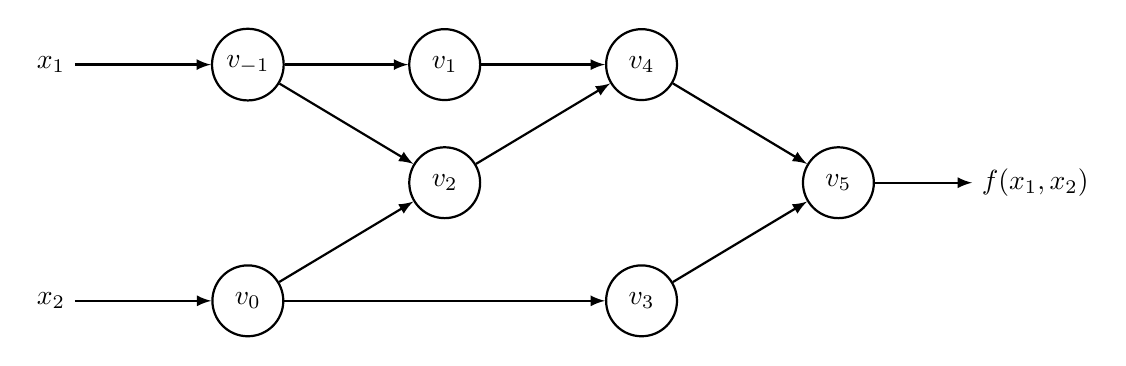
\begin{tikzpicture}[]
	
	\tikzstyle{vnode} = [circle,draw,thick,fill=white,minimum size=9mm]
	\tikzstyle{vedge} = [->,>=latex,thick]
	
	\node[vnode] (v-1) at (-8.5,0.5) {$v_{-1}$};
	\node[vnode] (v0) at (-8.5,-2.5) {$v_0$};
	\node[vnode] (v1) at (-6,0.5) {$v_1$};
	\node[vnode] (v2) at (-6,-1) {$v_2$};
	\node[vnode] (v3) at (-3.5,-2.5) {$v_3$};
	\node[vnode] (v4) at (-3.5,0.5) {$v_4$};
	\node[vnode] (v5) at (-1,-1) {$v_5$};
	
	\node[] (x1) at (-11,0.5) {$x_1$};
	\node[] (x2) at (-11,-2.5) {$x_2$};
	\node[] (f) at (1.5,-1) {$f(x_1,x_2)$};
	
	\draw (v-1) edge [vedge] (v1);
	\draw (v-1) edge [vedge] (v2);
	\draw (v0) edge [vedge] (v2);
	\draw (v0) edge [vedge] (v3);
	\draw (v1) edge [vedge] (v4);
	\draw (v2) edge [vedge] (v4);
	\draw (v3) edge [vedge] (v5);
	\draw (v4) edge [vedge] (v5);
	
	\draw (x1) edge [vedge] (v-1);
	\draw (x2) edge [vedge] (v0);
	\draw (v5) edge [vedge] (f);

\end{tikzpicture}
\end{document}
